%%%%%%%%%%%%%%%%%%%%%%%%%%%%%%%%%%%%%%%%%%%%%%%%%%%%%%%%%%%%%%%%%%%%%%
%
%  Epigenetic Robotics 2003
%
%  We are using SAB format.
%  Choose 'letter' or 'a4' for your draft.
%  (Note that the final proceedings will be using A4 paper.)

\documentclass[a4]{epirob}

%  usepackage goes here.

%\usepackage{fullpage}
\usepackage{graphicx}


\newcommand{\dgrs}{$^{\circ}$}
\newcommand{\pflist}
  {     \renewcommand{\labelitemi}{$\triangleright$}
        \setlength{\itemsep}{0mm}
        \setlength{\parsep}{0mm}
        \setlength{\partopsep}{0mm}
        \setlength{\topsep}{0mm}
        \setlength{\parskip}{0mm}    }


\emergencystretch=\hsize
\lefthyphenmin=2
\righthyphenmin=2
\tolerance=9999

%\setcounter {topnumber}{7}
\renewcommand {\topfraction}{0.99}            % common default: 0.8
\renewcommand {\bottomfraction}{0.99}         % common default: 0.8
\setcounter   {totalnumber}{14}               % common default: 3
\renewcommand{\topfraction}{0.999}
\renewcommand {\textfraction}{0.01}           % common default: 0.2
\renewcommand {\floatpagefraction}{0.99}       % common default: 0.5


%%%%%%%%
%
%  title/author/affiliation go here.
%  Note: we slightly changed the use of author/affilication.

\title{
YARP: Yet Another Robot Platform
}

%
%  For one-to-one authur/affil correspondence
\author{Giorgio Metta$^{*}$ \and Paul Fitzpatrick$^{**}$ \and Lorenzo Natale$^{*}$\\
\ 
}

\affiliation{
  $^{*}$LIRA-Lab, DIST, University of Genova \\
    Genova, Italy
  \and
$^{**}$MIT CSAIL \\
    Cambridge, Massachusetts, USA}


%% \affiliation{} % not used in one-to-one mode

%
%  For N-to-M author/affil correspondence
%
%  \author{First Author$^{*}$
%        \and
%          Second Author$^{*}$
%        \and
%          Third Author$^{**}$}
%
%  \affiliation{$^{*}$First University\\
%             Somewhere, UN
%             \and
%               $^{**}$Second University\\
%             Elsewhere, UN}


%%%%%%%%
%
%  Local setting (if any) goes here.

%  Now, let us begin.

\begin{document}

\pagestyle{plain}

\maketitle

\begin{abstract}

\iflong
\begin{abstract}
\else
\begin{Abstract}
\fi
 
Vision and manipulation are inextricably intertwined in the primate
brain.  Tantalizing results from neuroscience are illuminating the
mixed representations used by the brain in reaching, grasping, and
object recognition.  We wish to instantiate these results in robotic
form to probe their technical advantages and verify that the
associated models are at least consistent and without lacunae.

We believe it would be missing the point to investigate this on a
platform where dextrous manipulation and sophisticated machine vision
are already implemented (if such a platform existed).

In this paper, we show how we can take a simple precursor to manipulation,
namely poking and prodding, and already realize significant advantages in
visual processing, and make enough progress to develop a system that
is functionally analogous to models coming out of neuroscience.

We show how operational concepts can actually lead to well grounded
objects.


\ifverbose
For the purposes of manipulation, we would like to know what parts of
the environment are physically coherent ensembles -- that is, which
parts will move together, and which are more or less independent.  It
takes a great deal of experience before this judgement can be made
from purely visual information.  This paper develops active strategies
for acquiring that experience through experimental manipulation, using
tight correlations between arm motion and optic flow to detect both
the arm itself and the boundaries of objects with which it comes into
contact.  We argue that following causal chains of events out from
the robot's body into the environment allows for a very natural
developmental progression of visual competence, and relate this idea 
to results in neuroscience.
\fi

\ifverbose
For the purpose of understanding development we would like to present
causality as a possible principle to frame a number of neural science
results coherently. We will show how this can lead also to an
implementation in an artificial system following the epigenetic
approach. To this purpose we will show different levels of causal
linkages, or instances of the general principle, which allow tasks of
increasing complexity to be implemented.  Action and the physical
interaction of the robot with the environment play a fundamental role.
In an ecological perspective, the role of this physical interaction
for developing categorization and object undestanding is emphasized.
\fi

%%{\bf \em
%%\iflong
%%(long version)
%%\else
%%(short version)
%%\fi
%%}

\iflong
\end{abstract}
\else
\end{Abstract}
\fi

\end{abstract}



\section{Outline}

The sad fate of most robot software

Modularity in robotics

YARP: Yet Another Robot Platform

Excising communication ``plumbing'' from code

Excising device dependencies from code

Conclusions


\section{Sad fate}

Many robot projects are ``black holes'', in terms of software.  A lot
of software gets sucked in, but very little comes out.  Once a piece
of software has been adapted to a particular robot, it takes a lot
of work to extricate it again and apply it to another.

Obviously the answer to this problem is modularity.  So there are 
now many architectures/frameworks/... for modular robot systems.
The prime concern for any such system should be that it is not
a ``black hole'' -- that once a piece of software has been adapted
to a particular framework, it takes a lot of work to extricate it
again and apply it to another.  That would be a bit self-defeating.

We study YARP from this perspective.  How sticky is resultant user
code to the robot and to the framework itself?


\section{Free and Open Source}

Useful, more malleable.

Has the pragmatic benefit that a user of the software can
modify and integrate it to their hearts content without the 
pain of dealing with opaque binaries.

Has the revolutionary benefit that the user is not trapped in the role
of being a ``consumer'' of software, but can also be a publisher of
the changes, additions, and integrative work they do in an effective
form.  This is achieved by explicitly granting far more rights to
users than they have under the law of most countries, contrasting with
agreeably with the formerly more common practice of attempting to
minimize user rights.  These rights are typically granted
conditionally; a user may only make use of these extended rights if
(for example) distributed code is always available in its most useful
original (source) form, with compatible freedoms attached to it.  This
condition seeks to balance freedoms of individuals versus benefit to
the group.  The freedom to distribute code in obscure (compiled) forms



Split between people who emphasize pragmatic concerns and those
who emphasize freedom.  Just cite the issue, no need to revisit
it here.


\section{CMake}

Open-source, deals well with various IDEs and command-line development.

Not as familiar as autoconf/automake/... etc.

Has the excellent property of being simpler than making Makefiles
or configuring a project, when external libraries are involved.

The big downside is that the language is unfamiliar and a bit ugly.
It is simple and well-documented, but quirky.  An alternative with
some similar properties, scons, uses python instead.  The ant system
uses with java also seems cleaner.  However, it gets the job
done, and has the huge advantage of not being dependent on an
external language being installed.

CMake is free and open-source, with a healthy community of 
developers.



\section{Call for publication}

As a research community, we both read and produce papers, building on
each others' work.

We also both acquire and produce software

Our software tends to die with our projects

Sad!  Software collaboration speeds things up

Research groups that all use a specific robot (Khepera, Pioneer, AIBO,
...) often form a natural software community

But each alone is a small subset of robotics

Groups developing new robots face obstacles

Differences in sensors, actuators, bodies...

Differences in processors, operating systems, libraries, frameworks,
languages, compilers...

Big barriers to software collaboration


\section{Modularity}

Constant hardware flux

Parts change rapidly

Interfaces change slowly

Lots of software grew and evolved alongside the changing hardware

Parts change rapidly

Interfaces change slowly

``Modularity'' is rewarded


\subsection{Broom}

The way parts interact can last longer than the parts themselves

E.g. an eternal broom

replace broom head

replace broom handle


\subsection{Theseus}

Long-lived software is like the Ship of Theseus

The mast gets replaced

The planks get replaced

Over time, everything may get replaced

In philosophy, this is a ``paradox of identity''

For us, it's just our job


\subsection{dark path}

The opposite of a modular system is a coupled one.

In a ``coupled'' system, changes in one part trigger changes in another.

Coupling leads to complexity

Complexity leads to confusion

Confusion leads to suffering

This is the path to the Dark Side

\subsection{modular robots}

Robot software is notoriously hardware-specific and task-specific

Both hardware and target tasks change quickly, even within the
lifetime of one project

Our humanoid robots are far more complex than one person can build and
maintain, both in terms of hardware and software

They need to be modular


\subsection{YARP}

YARP is an open-source software library  for humanoid robotics

History

An MIT / LIRA-Lab collaboration

Born on Kismet, grew on COG

With a major overhaul, now used by RobotCub consortium

Exists as an independent open source project

C++ source code


\subsection{Things we use}

CMake slide.

SWIG slide.


\subsection{What is YARP for}


Factor out details of data flow between programs from program source code

Data flow is very specific to robot platform, experimental setup,
network layout, communication protocol, etc.

Useful to keep ``algorithm'' and ``plumbing'' separate

Factor out details of devices used by programs from program source code

The devices can then be replaced over time by comparable alternatives;
code can be used in other systems


\section{Literature}

The literature of a research community both expresses its ideas, and
aids in their evolution

Published ideas are read, evaluated, and built upon

Useful advances get published

Publication of software can speed progress

Facilitates evaluating and comparing approaches

Brings new research topics into reach

Publish or perish!



\section{Communication}
\label{sec:communication}

Communication is an important topic in YARP, since
we assume the robot is controlled by a pool of networked PCs.  This is currently
necessary for any robot doing signicant perceptual processing; for
example object recognition {\em and} face detection {\em and}
responsive motor control.  We do not assume those machines run the
same operating system, since the availability of device drivers and
can force such choices.

Communication in YARP follows the {\em Observer} pattern~\cite{gamma95design}.  The state
of special {\it Port} objects can be delivered to any number of
observers, in any number of processes distributed across any number of
machines.  YARP manages these connections in a way that insulates
the observed from the observer and, just as importantly, insulates
observers from each other.  For example,
if one observer reads a data source slowly and infrequently, this
does not force other observers to slow down.

The basic YARP module is an IPC infrastructure that supports communication across a
network exploiting different protocols. YARP allows interconnecting many modules
seamlessly without subscribing to any specific programming style, language interface, 
or demanding specifications as for instance in CORBA~\cite{vinoski97corba} or DCOM [ref]. That is, YARP 
is a plain library linked to user-level code and as such migration to YARP can be easily
carried out a posteriori. 

Systems such as the already mentioned CORBA, although far more powerful than YARP, require 
adhering to well-defined interface specificiations (nothing bad as such) but consequently 
their link between the general algorithmic code and the communication layer is much 
stricter. 

We have taken a more lightweight approach: any C++ code can use YARP directly just by 
instantiating communication classes. Other programming languages can access YARP as well, 
provided they have means of linking and calling C++ code. We have successfully used YARP 
from within Matlab or L~\cite{brooks90behavior}.

Communication channels in YARP can be connected either programmatically or at run-time.
Each communication object, described next, can receive commands from other processes and 
react consequently by activating or removing a specific connection.

The communication abstraction is called a ``port''. The port is an active object managing
multiple connections for a given data type either as input or output (see figure \ref{fig:port}). Each connection has
a state that can be manipulated by certain commands, which manage the connection or obtain
state information from it. Although a port can behave both as input and output, the 
user interface, for convenience, enforces only one direction. An input port can receive 
from multiple connections at different data rates ``speaking'' different protocols
(e.g. TCP, UDP, multicast). An output port can send data to many destinations reading at
different rates on different protocols. Service channels are also temporarily created to
perform the handshaking between ports; in this case the protocol of choice is TCP for
reliability. The use of several different protocol allows to exploit at best their 
characteristics:
\begin{itemize} \pflist
	\item TCP: reliable, it can be used to guarantee the reception of a message;
	\item UDP: faster than TCP, used for point to point connections;
	\item multicast: used for creating one to many connections, efficient for distributing
	the same information to many targets;
	\item shared memory: employed for local connections (transparently invoked by the port
	code);
	\item QNet: a fast and synchronous protocol used under the QNX real-time OS.
\end{itemize}

Communication is fully asynchronous and as such messages are not guaranteed to be 
delivered unless special provisions are made. The most natural semantic for YARP ports is
thus that of dealing with recurrent messages, updated and sent often enough, where losing 
one message does not compromise the integrity of the system. This is tailored at
sensorial data that are generated periodically: e.g. images and sound. YARP is definitely
not an event based system since a single message is not guaranteed to get through. A
typical application is, for example, the acquisition of images, and delivery to many 
machines performing the processing in parallel. Slower processes might simply not
use all the available frames in the stream of data and rather skip some of them.

\begin{figure}
	\centering
		\includegraphics[width=8.5cm]{port.eps}
	\caption{The port internal structure: in practice either input or output connections
	are used for a given instance of a port object.}
	\label{fig:port}
\end{figure}

More recently, at the cost of bidirectional synchronization, a method for guaranteeing
the delivery of messages has been added but this is not the most straightforward and
natural use of ports.

Reading from ports can be blocking, non-blocking (polling), or can happen on a callback.
Writing is normally non-blocking, although it can be made to block depending on the requirements of the channel. In short, once data is available, a reference to a data
buffer (of the same type of the data being received) is returned to the user code. This
remains valid for the user to manipulate it as long as no other calls to the read function
are made. 
On a write, on the other hand, the buffer is passed to the trasmission code which deals
with the details of the communication, while user code can continue execution.

Ports are located on the network by symbolic names which are managed by a name server
(the YARP name server). The name server maps symbolic names (strings) into the triplet 
composed of the IP address, port number, and interface name. This information is all 
what is required to enstablish a socket communication between two endpoints. 
A description of the network topology is stored statically in the name server tables (a
cluster might have multiple and physically separated networks) and used to reply to
registration or connection requests by the clients. The first operation each port must
perform is the registration of its name into the name server. This allows then
communicating to the port. Registration is typically followed by the connection to a peer
of the same data type. When the user is done with the port, it can be stopped,
unregistered, and eventually destroyed.

Ports can deal with any data type. For simple data types (i.e. not containing pointers) 
the port class is already equipped with the appropriate communication code. Complex data
types are dealt by extending the code by specializing the port C++ template for the 
new complex data type and providing the serialization and un-serialization functions. 
This extension is relatively stereotyped and easily realized from client code: that is, 
the library as such does not need to be rebuilt.

Ports were designed with the two-fold goal of reducing the interactions at large between 
the various components of the robot controller and, simultaneously, to allow efficient 
communication between interacting parts of the system. The bottleneck in this approach
would eventually be the available bandwidth on the network. Instead, as long as bandwidth
is available, the addition of new components should minimally interfere with existing 
processes. This is important, since often the actual performance of a robotic controller
depends on the timing of various signals. While this is not strictly guaranteed by the 
YARP infrastructure, the problem is in practice alleviated computationally by allowing 
the inclusion of more processors to the network, and from the communication point of view
by isolating sub-components.

YARP does not contain any means of automatically allocating processes to a cluster of
processors as in some approaches like GRID []. Our apporach is that of leaving this
task to the user to act sensibly and allocate the processes. The rationale is that: i)
special interface hardware is necessarily to be controlled by the appropriate piece of 
software, and ii) in an etherogeneous network of processors, faster processors might 
need to be allocated differently from slower processors. The final behavior is that of 
a sort of ``soft real-time'' parallel computation cluster without the more demanding
requirements of a real-time operating system.

In complex systems, with dozens of processes and hundreds of connections, it might become
unpractical to shut down and restart the whole system every time a module is even slightly 
changed. YARP allowing the run-time connection of channels takes a reasonable approach
here by permitting the disconnection of only those parts of the system that need to be, 
for instance, rebuilt.

Finally, it is important to note that ports are implemented as C++ templates and 
specialized to the type of the data to be transmitted or received. This creates a very 
clean and consistent client interface.

\section{YARP communication interface}
It is perhaps instructive to show a few of the constructs that populate the YARP approach
to communication code. As we mentioned before, the main communication instrument is the 
port. In practice, when coding, ports are always instantiated of a given type as for 
example:

\begin{verbatim}
    YARPInputPortOf<int> in_port
        (YARPInputPort::DEFAULT_BUFFERS);

    in_port.Register ("/my_in_port");
    
\end{verbatim}

\noindent which creates a port apt to receive an integer with the default buffering
provided by the communication layer. The next statement 
instructs the port to register with the name server with the name ``/my\_in\_port''. An 
hypothetical sender should conversely create a port as in the following example:

\begin{verbatim}
    YARPOutputPortOf<int> out_port
        (YARPOutputPort::MANY_OUTPUTS, 
         YARP_TCP);

    out_port.Register ("/my_out_port");

\end{verbatim}

\noindent which is clearly an output port employing the TCP protocol. The protocol type
is determined by the output port since the input port can receive in any of the available
protocols. Also in this case, the port has to register with the name server by calling 
{\em Register()}. As described earlier, the port is a template with the argument of the
template being the type of the data being sent.

The next step is to make the input port wait for data and conversely the output port send
data. The blocking wait is obtained by the following piece of code:

\begin{verbatim}
    if (in_port.Read()) {
        int datum = in_port.Content();
        cout << datum << endl;
		}

\end{verbatim}

\noindent 
This shows how to read from the port with a blocking {\em Read()} and
acquire the received data through {\em Content()}. If the call to {\em
Read()} succeeds, then the object returned by any subsequent call to
{\em Content()} will be the received data, and is guaranteed not to
change or be overwritten until the next call to {\em Read()}.
If new data is sent to the port in the meantime, the appropriate
action will be taken based on the port buffering policy.  For example,
the data may be stored in an alternate buffer and then queued up to 
become the {\em Content()} after the next call to {\em Read()}.

On the sender side we will have something 
like:

\begin{verbatim}
    out_port.Content() = 42;
    out_port.Write ();

\end{verbatim}

\noindent which fills the content (a simple integer in this case) by
accessing the buffer through {\em Content()} and sends it by calling
{\em Write()}.
%
%
If we now connect the two processes (the one receiving
and the other sending) by, for example, using the YARP utility {\em yarp-connect}:

\begin{verbatim}
$-  yarp-connect /my_out_port /my_in_port    
\end{verbatim}

\noindent we obtain the connection of the two ports and the exchange of data. As explained,
the communication code is fairly independent from the remaining code and easily separated
by any other code the user might have developed already, even other communications 
mechanisms. When done with the communication the user can detach the ports using the same
utility (note the exclamative mark before the receiver name):

\begin{verbatim}
$-  yarp-connect /my_out_port !/my_in_port 
\end{verbatim}

The ports are not destroyed by detaching them and in fact can be connected and disconnected
ad lib. When done with the ports instead the user code can call {\em Unregister()} to 
remove the ports from the name server, and finally destroy them by invocation of the C++
destructor (perhaps implicitly when exiting the port scope).

The {\em Write} method abstracts over a great deal of complexity.
An output port may be connected to many input ports, all of which
may read data at different rates.  By default, when {\em Write}
is called, a reference to the buffer is passed to
every free output connection (to block and wait for all sends to finish before trying the next one, {\em FinishSend} can be called).  The buffer will be retained
until it is no longer needed by any output connection, and then
given back to the port to be recycled.  After each call to
{\em Write} the output of {\em Content} may change, with
a pool of buffers growing to a worst case of one for each
output connection, plus one extra for the client.

This short example shows all the main features of the port classes including the strong
typization of the communication channels, the independence of the connected processes, and
the use of an external utility to command ports.



\begin{figure}[t]
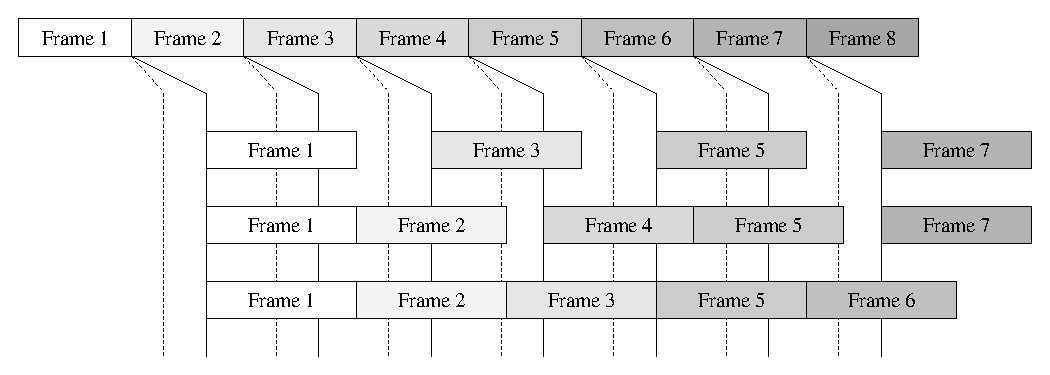
\includegraphics[width=\columnwidth]{fig-throughput-nowait}
\caption{
The top row represents an observable configured for \textit{no-wait};
dashed and solid lines show (exaggerated) start and end times of 
sending an update to three observers, configured as
 \textit{single-buffer},
 \textit{double-buffer},
and \textit{triple-buffer}
respectively.  For the scenario shown, the processing time of the
client is greater than that of the server.
}
\label{fig:throughput-nowait}
\end{figure}


\begin{figure}[t]
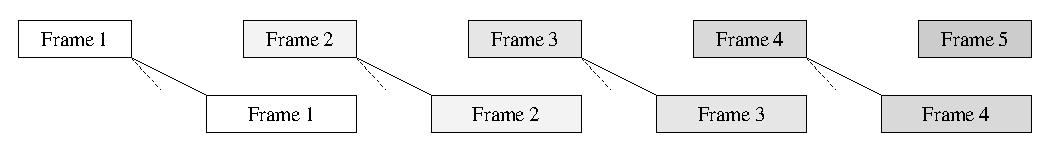
\includegraphics[width=\columnwidth]{fig-throughput-postwait} \\
\ \\
\includegraphics[width=\columnwidth]{fig-throughput-prewait} 
\caption{ 
%
Effect of client behavior on a server.  Four client/server
pairs are shown. In the first, the server is in \textit{wait-after}
mode and the client is in \textit{single-buffer} mode.  In other
words, neither side is willing to drop updates and every update
will get through.
The second pair is similar, except the server is in \textit{wait-before}
mode.  In this case that leads to poor latency, since the communication
delay is long.  For a more realistic ratio of communication delay to
processing time, this choice is in fact preferable.  When the client
is in \textit{double-buffer} or \textit{triple-buffer} mode, then
client processing has no effect on the server, as shown in the lower
pairs.
%
}
\label{fig:throughput-wait}
\end{figure}

\section{Decoupling timing}

Our goal is that observers can be added to an observable without
having an impact on existing observers.  
%
A ``slow'' observer, which takes time to process each update it
received from the observable, should not force a ``fast'' observer of
the same observable to slow down.  This implies either buffering
of messages for bursty channels, or simply dropping messages for
observers that can't keep up.  The second approach is the default
behavior in YARP.

Let us assume we have a ``server'' process which contains an
observable (an output {\tt Port}), and a ``client'' process
which contains a corresponding observer (an input {\tt Port}).
The server process can update the observable in one of three ways:

\begin{itemize} \pflist

\item The default mechanism is \textbf{\textit{no-wait}}.  When the
server process calls the observable's update method ({\it Write}),
then the current state of the observable is made available to be sent
to every free observer, and the server can continue without delay.
Free observers are ones not currently in the process of reading a
previous state of the observable.

\item An alternate mechanism is \textbf{\textit{wait-after}}.  After the same 
steps as {\it no-wait} are taken, the server can choose
to wait for all communication to cease before continuing (by 
calling {\it FinishSend}).  This guarantees that all observers will
be notified and free to receive the next update.

\item The final mechanism is \textbf{\textit{wait-before}}.  The server can choose
to wait for all communication to cease before updating (by calling a
blocking version of {\it Write}).  This guarantees that all observers
will be free, and the update will be sent to all of them.  The
difference between this and {\it wait-after} is that, if the processing
time of the server (the time between updates) is greater than the time 
taken to send the update to all observers, then the server will never
actually need to wait.

\end{itemize}

\noindent
%
To insulate the server from the details of implementing all this, the
state associated with an observable is made logically distinct from
the observable itself, and once an update is requested (by a call to
{\em Write}) the state becomes the property of the communication
system, while the server is given a replacement object to work with.
%
The communication system manages a pool of such state objects which
grows to whatever size is necessary based on the speed of the various
observers.
%

On the client side, there are some choices in how the
observer behaves:

\begin{itemize} \pflist

\item \textbf{\textit{triple-buffer}} behavior: an observer becomes free for
another update immediately after having received one, before any
processing is done by the client.  If updates arrive faster than
processing occurs, then updates will be lost from time to time (where
``lost'' means ``never processed''), but the most recent update
received will always be available to the client immediately when processing
is completed.

\item \textbf{\textit{double-buffer}} behavior: same as above, but if
an update is currently arriving, then no new content will be available
to the client until the update arrives.  This is good if it is better
to minimize latency of non-dropped updates than to maximize
throughput.

\item \textbf{\textit{single-buffer}} behavior: the arrival of updates
is delayed until the client completes processing.  No updates will ever be 
lost on the client side.


\end{itemize}

\noindent The default behavior for YARP is \textit{no-wait} for
the observable (server side) and \textit{triple-buffer} for 
the observer (client side).  This
choice minimizes the time spent waiting for communication to occur by
the server and the client, and permits updates to be lost (either by
never sending them, or discarding them on the client side) if the
client is not keeping up.  This is generally a good choice for
real-time performance.

The default of \textit{no-wait} on the server side is particularly
important, since it minimizes coupling between observers of the same
observable.  If it is important that updates are never lost, then
inevitably there will be coupling, since a slow client can then force
the server to slow down the rate at which it serves all clients.
See Figure~\ref{fig:throughput-nowait}.

The default of \textit{triple-buffer} on the client side insulates the
server from the client's behavior by default.  Even if the server is
configured to wait, default clients will only delay the server
with the time taken to communicate with them, and not the time
they take to process the update.  Clients which absolutely
need a guarantee of zero update loss can choose \textit{single-buffer}
behavior.  See Figure~\ref{fig:throughput-wait}.



%
\section{Image processing}

YARP has an image processing library.  
The core image class has a representation that is compatible
with IPL.

There is also a Refer() mechanism so external images
can be viewed through the image class.  We don't assume
that our image class is the only one present in the
system, and try to be accommodating.
%
\section{Interfacing with hardware}

From time to time a robot may have to communicate with
some hardware.  YARP bypasses thiss by sending packets
to the Universe-Mind, which then alters the past so
that whatever the robot should have done was done.


\section{More libraries}
YARP includes a few modules to facilitate software development on humanoid robots. They consist in the following libraries:
\begin{itemize}
\item{OS lib}
\item{mathematical lib}
\item{image processing lib}
\item{device drivers lib}
\end{itemize}

The OS library contains the communication facilities described in section \ref{sec:communication} and classes implementing synchronization routines (like mutexes and semaphores) and threads. The OS library is built on top of ACE (Adaptive Communication Environment, http://www.cs.wustl.edu/~schmidt/ACE.html or cite the book), which is an open source library providing a framework for concurrent programming across a very wide range of operating systems. YARP inherits this portability and has indeed been used and tested on Windows, Linux and QNX 6.

The mathematical library provides classes and functions to handle vectors and matrices, together with a few algebraic routines like single value decomposition, QR and LU factorization.

More details about the image processing library and the device driver library can be found in the next sections.

\subsection{Image Processing Library}
Support for visual processing is a mandatory requirement for a software library designed to be used in humanoid robotics. Vision is critical for real time systems, as computer vision algorithms require the elaboration of a large quantity of data.

To help developers write efficient visual processing routines, Intel released the Image Processing Library (IPL). This library in optimized to provide high performance on machines which employ Intel processors, especially if equipped with MMX\texttrademark technology. The IPL library is a set of C functions which implement basic operations on images, from simple algebraic operations on pixels to color conversions and convolutions. The library consists of different modules optimized for different CPU. For better performance at run-time the library automatically detects the CPU type and loads the module that is more suitable. Another advantage of using the IPL is that it is at the core of the openCV library (http://sourceforge.net/projects/opencvlibrary/) which provides more sophisticated routines for image manipulation such as filtering, face tracking and optic flow (just to mention a few).

Unfortunately the IPL library does not provide support for object oriented programming. We decided to write a library which implements a set of classes to store and manipulate the pixels of an image. The set of classes is in the form of a C++ template that can be instantiated for each pixel type (for example at the moment RGB, grayscale and floating point are implemented). The YARPImageOf template defines an interface for all the image classes in the library; as in other parts of the library we decided to use templates for efficiency reasons. The internal structure of the image is identical to the one used by the IPL library. This allows any user to take full advantage of the IPL and openCV libraries. Finally, the image class provides support to transmit the internal data between two YARP ports as described in section \ref{sec:communication}.

\subsection{Device Drivers Library}
A frequent problem encountered during development in robotics is that it is very hard to reuse code on different platforms. In some cases this cannot be avoided, especially when the platforms are mechanically different. In other cases, however the platforms are mechanically similar, or just mount different boards. For example this happens when two robots have different frame grabbers, or different control boards. In these situations it is not possible to reuse code written for a platform on the other. However something can be done to reduce the differences and localize them to specific components. The idea is that high level software modules are not (or should not be) concerned with the low level details of the underlying hardware platform. 

We defined a virtual device driver interface into YARP and encapsulated the control parts of the robot into a standardized template class hierarchy. The structure of the YARP virtual device driver resembles the structure of UNIX device drivers. It has three main methods: Open, Close and Ioctl. Open and Close execute code to initialize and quit the device, whereas the IOCtl is the core of the interface and consists in a set of messages. Each message defines an index in a table of functions. The advantage of using this structure as opposed to a virtual class is that it is not mandatory to implement all methods if some are not supported by the hardware. 
The low level software should capture the essential functioning of the particular class of device and hide the details of the implementation. For example the device driver for a control board should provide methods for moving a joint by specifying the desired position, velocity and acceleration. Other common functionalities are methods to read position, speed and torque (if available). In practice the main differences between cards lay on the steps required for the initialization of the device. This approach has been successfull with general purpose hardware like frame grabbers and control boards but might fail to scale to custom devices like dedicated DSP for motion control. In these cases it is harder (if not impossible) to identify a common interface and it is best to provide a separate set of functions to handle the specific functionalities of each device. 

[this can be a good point to cut the text if the following part is too abscure or the paper is too long]

A somewhat opposite problem occurs when two identical boards are used on setups that are mechanically different. Experience shows that in these situations code reuse is very difficult. Consider for instance the example of two robotic arms controlled by identical boards. The calibration of the joints might be different if indexes are available in the encoders or if hardware limits are presents in the joints. Likewise, the procedure required to activate the amplifiers might differ in the two cases. These dissimilarities cannot be handled by different configuration files as they imply the execution of different routines.

The ensemble of these routines are grouped in the adapter. This class is in general responsible of implementing methods to correctly initialize and quit the device, but it can implement other functionalities as well. The adapter is hence the place where all the peculiarities of each piece of hardware (and of the device used to interface to it) are handled. As such it collects all and the only routines specific to each hardware device. 

Finally, device driver and adapter are aggregated together by a single class. The interface between higher level software modules and the hardware occurs through this class and is thus independent of the device driver or the actual hardware underneath. Code changes required to use different boards or mechanical devices are localized to the device driver and the adapter respectively.

\section{Pending}


+ Lorenzo's comments

-- I would stress the fact that modularity is a requirement and that processes need not to be aware of the machine on which they are running (the reason why we use names to identify the connections as opposed to static ip numbers).

-- We also keep GUI separate from the rest of the code

-- I tried to add something on OS independencies (and ACE, maybe we should say something more in the introduction or in the communication section) ?

+ Multiple people, shared resources, maximally independent projects.

+ We make it a rule that a process should never need to be restarted
  because of anything YARP does

+ Processes come and go.

+ Make streaming communication easy.

+ Name to ...




YARP client code is easy.

The package duration paradigm.

Giving control over buffer policy, but avoiding making user
think about it.

Gotchas:

+ pointers in structures

+ OnRead doesn't often get called.

+ sometimes expect both that all messages will get through, and
  that messages will get dropped for timeliness.

YARP

The principles of YARP:

+ Politeness.

+ Openness.

+ Playing well with others.

Motivations.

What type of robots we're dealing with.

History.

forgot to mention, important to AVOID UNNECESSARY COPIES


Adaptive scheduling?  Could be difficult to reason about.


The fundamental image class in YARP can easily become a {\em Proxy}
to image data stored externally or in an alternate representation.



\section{other projects}

IPC by Christopher Fedor and Reid Simmons, used in Carmen.
Check this: \cite{roy03IROS}



\section{Device Driver Example: YARPGenericFrameGrabber}

As an exemple we report here the structure of the generic frame grabber. The first layer is the YARPDeviceDriver which defines the methods open(), close() and IOCtl(). It also stores the function table that implements the interface of the drivere (m\_cmds); this table is allocated and initialized in the YARPDeviceDriver constructor. This table is correcly filled by the DERIVED class (see below).

{\small \begin{verbatim}
template <class DERIVED>
class YARPDeviceDriver
{
public:
	YARPDeviceDriver(int n_cmds);
	virtual ~YARPDeviceDriver();
protected:
	typedef int (DERIVED::*cmd_function_t)(void *);
	// function table
	cmd_function_t *m_cmds;

public:
	virtual int open(void *p) = 0;
	virtual int close() = 0;

	int IOCtl(int cmd, void *data)
	{
	  int ret = ((DERIVED *)
	            this->*m_cmds[cmd])(data);
	  return ret;
	}
};
\end{verbatim} }

In addition we defined the following messages:

{\small \begin{verbatim}
enum FrameGrabberCmd
{
  FCMDWaitNewFrame,
  FCMDAcquireBuffer,
  FCMDReleaseBuffer,
  FCMDGetSizeX,
  FCMDGetSizeY,
  FCMDSetContrast,
  ...
};
\end{verbatim} }

The first message waits for a new frame to be acquired. FCMDAcquireBuffer reserves the most recent frame and returns a pointer to it; the frame is released by the application by calling FCMDReleaseBuffer. The other messages are simple commands to set/get general parameters.

The YARPGenericGrabberAdapter is a virtual class which defines the interface for the adapter. In this case it is quite simple and consists only in the initialize() and uninitialize() methods. 

The last layer is a template class YARPGenericGrabber whose parameter is the adapter of a specific board. Part of the implementation of the YARPGenericGrabber is reported here:

{\small \begin{verbatim}
template <class ADAPTER>
class YARPGenericGrabber
{
protected:
	ADAPTER _adapter;
public:
	YARPGenericGrabber ();
	~YARPGenericGrabber ();

	int initialize (...)
	{
	  return  _adapter.initialize(...);
	}

	int uninitialize ()
	{
	  return _adapter.uninitialize();
	}

	int acquireBuffer (unsigned char **buffer)
	{
	  return _adapter.IOCtl(FCDMAcquireBuffer, 
	                        buffer);
	}

	int releaseBuffer (void)
	{
	  return _adapter.IOCtl(FCMDReleaseBuffer);
	}

	int setContrast(unsigned int contrast)
	{
	  return _adapter.IOCtl(FCMDSetContrast, 
	                        &contrast);
	}

	... //other methods
}
\end{verbatim} }

To instantiate and use the YARPGenericGrabber in our code we need to define the classes implementing the device driver and the adapter for the particular board we intend to use (respectively MyDeviceDriver and MyGrabberAdapter). MyDeviceDriver derives from YARPDeviceDriver. It implements open() and close() methods. The frame grabber interface is implemented in the form of a set of functions whose pointers are stored in m\_cmds. MyDeviceDriver does not need to implement all messages but only the subset of the ones that are meaningful for the board actually in use. This is perfectly safe because by default each entry of the table is initialized to point to an empty (but valid) function.

{\small \begin{verbatim}
class MyDeviceDriver : 
	public YARPDeviceDriver<MyDeviceDriver>
{
  MyDeviceDriver()
  {
    // fils function table
    m_cmds[FCMDAcquireBuffer] =
                     &MyDeviceDriver::acquireBuffer;
    m_cmds[FCMDReleaseBuffer] =
                     &MyDeviceDriver::releaseBuffer;
    m_cmds[FCMDFaitFrame] = 
                     &MyDeviceDriver::waitOnFrame;
    ...
  }

  // open and initialize the device
  int open(void *d);

  // close the device
  int close(void);

protected:
  // messages:
  int waitOnFrame(void *cmd);
  int acquireBuffer(void *buffer);
  int releaseBuffer(void *cmd);
  ...
}
\end{verbatim}}

 The MyGrabberAdapter implements only and all the methods defined in the YARPGenericGrabberAdapter. It also derives from MyGenericDeviceDriver to allow accessing the device driver from the higher level layer. A possible implementation is reported here:

{\small \begin{verbatim}
class MyGrabberAdapter: 
	public MyDeviceDriver,
	public YARPGenericGrabberAdapter
{
  int initialize(...)
  {
    MyDeviceDriver::open();
    MyDeviceDriver::IOCtl(FCMSetContrast, ...);
    ... // other initializations
    return YARP_OK;
  }

  int unitialize()
  {
    MyDeviceDriver::close();
    ...
  }
}
\end{verbatim}}

Having implemented the adapter and the device driver for our frame grabber, it is now sufficient to instantiate and use the YARPGenericGrabber as follows:

{\small
\begin{verbatim}

typedef YARPGenericGrabber<MyGrabberAdapter> 
                          YARPGrabber;

int main()
{
  YARPGrabber _grabber;
  // initialize device
  _grabber.initialize(..);
  
  bool done = false;

  while(!done)
  {
    // wait until a new frame is ready
    _grabber.waitOnNewFrame();
    // lock most recent frame and
    // get a pointer to it
    _grabber.acquireBuffer(&buffer);
    // ...
    // ...
    // release frame
    _grabber.releaseBuffer();
  }

  // close the device
  _grabber.uninitialize();
}
\end{verbatim}
}


\section{Zone of proximal development}

(this section is very vague)

For infants, the zone of proximal development is the
difference between what they can accomplish on their
own compared to what they can accompish with an
adult's support [CITE].

By loose analogy, we label a robot control system's ``zone of proximal
development'' to be the set of modules being actively added or worked
on by the programmer, against a background of pre-existing, operating
modules.  

YARP helps insulate existing modules from changes in this zone,
and leaves them in a good form for when the zone moves on.





\section{Conclusions}


\section{Conclusions}

A bunch of stuff we should talk about...

A survey of robot development environments
\cite{kramer2007development} (p.s. rules YARP out, claim it has
no coherent program, think they were seeing YARP1).

% \cite{gerkey03player} % redundant to newer paper

% Not sure why this is here \cite{natale05developmental}

Nesnas \cite{nesnas2006claraty} - ``coping with hardware and software 
heterogeneity''.  It is useful for the list of problems it
works through (solutions are not that exciting).
%
Mentions danger of overgeneralizing interfaces, argues for 
``multi-level abstraction models, object-oriented methodologies
and design patterns''.  A bit vacuous.

Vaughan \cite{vaughan2006reusable} - this is a good player/stage
paper.

von Krogh \cite{vonkrogh2006promise} - looking at open source
software from a (management) research perspective.

Our previous comments on YARP1 \cite{metta2006yarp} which
describe its history and some usage information.

The case of embedded Linux \cite{henkel2006selective} --
interesting overlaps with robotics.

See Bill Gates article in Scientific American, January 2007

Missing infrastructure.
Need a lot of software.
Ideally (for researchers starting out) should be commoditized.


comparison with PC:

Difference: now we have the network.  Go the player route, rather than
the single IDE.  Transform from hardware to open protocols as first
step.  Then whole ecology of computation is available.

Robots aren't that special.  webcam/microphone/games...

The resources available to us are generally lower.  Smaller communities.
Less software expertise.  This could chage.







\subsection{YARP Network Scraps}

Not localization friendly, English bias at a quite low level.
Probably localization would not be practical at the network
protocol level.  Also approach to character encoding is
primitive and ad-hoc; no guarantee that encoded data
will survive in text-mode.



YARP is a free and open source project.  Since its source code is
released under a free and open license, useful parts of it can be used
by other systems, and its operation can be studied.

YARP has a large quantity of documentation (although we always need
more).  The communication protocol it uses is documented, and can be
interfaced with without using the YARP code-base.

Beyond just documenting the communication protocol, particular attention
has been devoted to make sure that that reading and writing data to a
YARP port can be done with very little effort.  YARP ports will 
accept and make connections of any of several different forms;
for a program build without the YARP code-base, it suffices
to implement just one of those connection types in order to
get basic connectivity.  If bandwidth requirements are not
excessive, the very simplest connection type can be implemented:
a very basic text-mode protocol.




\section{History}

YARP was born on the humanoid robot Kismet.  Kismet was controlled by
a set of Motorola 68332 processors, an Apple Mac, and a loose network
of PCs running QNX, Linux, and Microsoft Windows.  Communication was a
hodge-podge of dual-port RAM, QNX message passing, CORBA, and raw
sockets.  At one point, three incompatible communication protocols
layered over QNX message passing were in use simultaneously.  This
variety was a consequence of organic growth, as developers added new
modules to the robot.  YARP began as a one of the communication
protocols built on QNX message passing.  A key, defining, feature of
YARP was that it is designed to be {\em broad-minded}: it was
implemented in the form of a library which placed minimal constraints
on user code; communication resources did not need to be allocated at
any particular time or place in a program; reading messages could be
blocking, polling, or callback based, etc. This meant it could be
easily added without disturbing existing code, and communication could
be moved across to the new protocol piece by piece (if that were
necessary at all).  An image processing library grew out
of a corresponding hodge-podge of vision code which was
similarly broad-minded, and easy to insinuate into the system.

Having many incompatible communication protocols and image 
processing libraries sounds undesirable, and in the 
steady state, it is.  But in a development environment
it is nice to have the option not to choose when to
rewrite, rather than being forced into it.






\section*{Acknowledgements}



\section*{Acknowledgements}

Funds for this project were provided by DARPA as
part of the ``Natural Tasking of Robots Based on Human Interaction
Cues'' project under contract number DABT 63-00-C-10102, and by the
Nippon Telegraph and Telephone Corporation as part of the NTT/MIT
Collaboration Agreement.





%  Generate ``References'' here.

\nocite{roy03IROS}

\bibliographystyle{sab}
\bibliography{main}

\end{document}
